
\begin{figure}[htb]
	\centering
	\def\mylength{.35\linewidth}
	\def\myscale{2.5}
	\begin{subfigure}[b]{\mylength}
		\centering
		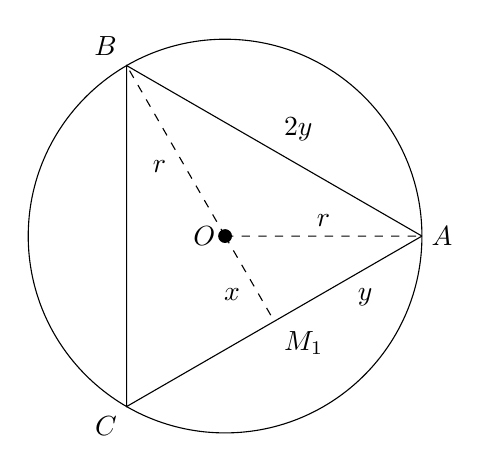
\begin{tikzpicture}[scale=\myscale]
			\draw(0,0)coordinate(O)node[left]{$O$}circle(1cm);
			\draw(1,0)coordinate(A)node[right]{$A$}
				--(-.5,{.5*sqrt(3)})coordinate(B)node[above left]{$B$}
				node[midway,above right]{$2y$}
				--(-.5,{-.5*sqrt(3)})coordinate(C)node[below left]{$C$}
				--(A)node[pos=.75,below right]{$y$};
			\coordinate(M)at(.25,{-.25*sqrt(3)});
			\draw[dashed](O)--(A)node[midway,above]{$r$}
				(O)--(B)node[midway,below left]{$r$}
				(O)--(M)node[below right]{$M_1$}node[midway,below left]{$x$};
			\fill(O)circle(1pt);
		\end{tikzpicture}
		\caption{}
	\end{subfigure}~%
	\begin{subfigure}[b]{\mylength}
		\centering
		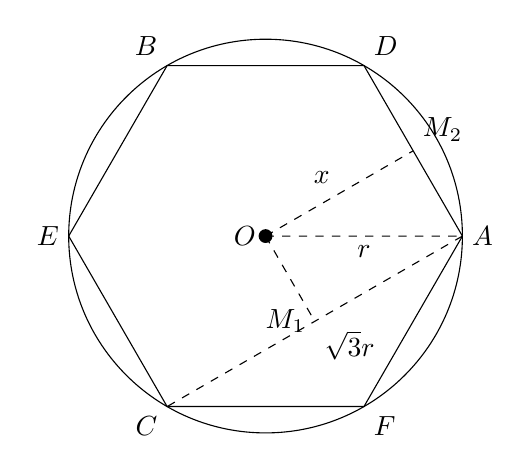
\begin{tikzpicture}[scale=\myscale]
			\draw(0,0)coordinate(O)node[left]{$O$}circle(1cm);
			\draw(1,0)coordinate(A)node[right]{$A$}
				--(.5,{.5*sqrt(3)})coordinate(D)node[above right]{$D$}
				--(-.5,{.5*sqrt(3)})coordinate(B)node[above left]{$B$}
				--(-1,0)node[left]{$E$}
				--(-.5,{-.5*sqrt(3)})coordinate(C)node[below left]{$C$}
				--(.5,{-.5*sqrt(3)})node[below right]{$F$}
				--(A);
			\draw[dashed](O)--(.75,{.25*sqrt(3)})coordinate(M)node[above right]{$M_2$}
				node[midway,above left]{$x$}
				(O)--(A)node[midway,below]{$r$}
				(O)--(.25,{-.25*sqrt(3)})node[left]{$M_1$}
				(A)--(C)node[midway,below right]{$\sqrt3 r$};
			\fill(O)circle(1pt);
		\end{tikzpicture}
		\caption{}
	\end{subfigure}
	\caption{}
\end{figure}

如图,易见\(\triangle AOM_1\)与\(\triangle BAM_1\)相似,
于是可以根据勾股定理和相似三角形建立关于\(x\)和\(y\)的方程\[
	\left\{ \begin{array}{l}
		(r+x)^2+y^2=(2y)^2, \\
		\frac{y}{x}=\frac{r+x}{y}, \\
		x,y,r>0,
	\end{array} \right.
\]
化简得\[
	\left\{ \begin{array}{l}
		(r+x)^2=3y^2, \\
		y^2=x(r+x), \\
		x,y,r>0,
	\end{array} \right.
	\quad\text{或}\quad
	\left\{ \begin{array}{l}
		(r+x)^2=3x(r+x), \\
		x,y,r>0,
	\end{array} \right.
\]
于是有\(r+x=3x\),
解得\(x=\frac12 r, y=\frac{\sqrt3}2 r\).
